\chapter{Implementacja}
\label{cha:impl}

Rozdział zawiera odwzorowanie konceptu przedstawionego w rozdziale trzecim na kod aplikacji OffCalendar, zarówno po stronie klienta, jak i serwera. 

Prześledzono technologie i biblioteki użyte podczas tworzenia interfejsu graficznego, mechanizmy odpowiedzialne za manipulację wydarzeniami, przedstawiono rozwiązanie kwestii automatycznej detekcji stanu połączenia internetowego oraz synchronizacji danych. Opisano również komunikację z bazą danych oraz implementację bezstanowych interfejsów niezbędnych do zachowania integralności części klienckiej oraz serwerowej.

Zastosowane rozwiązania zostaną poparte szczegółowymi objaśnieniami w postaci kodu oraz wzbogacone grafikami i schematami przedstawiającymi wygląd aplikacji docelowej.


\section{Aplikacja kliencka}
\label{sec:apKli}

Główną część projektu OffCalendar stanowi aplikacja kliencka. Do jej zadań należy gromadzenie danych użytkownika w pamięci podręcznej przeglądarki, komunikacja z częścią serwerową celem dokonania autoryzacji i synchronizacji oraz reagowanie na stan połączenia internetowego. 

Konieczność pełnego wsparcia dla trybu online determinowała konstrukcję interfejsu graficznego a format gromadzonych danych (wydarzenia) podyktował rodzaj technologii lokalnego przechowywania danych.

\subsection{Interfejs graficzny}
\label{sec:intGraf}

Podstawowym założeniem systemu jest możliwość wykonywania wszystkich operacji niezbędnych do zarządzania wydarzeniami bez dostępu do sieci Internet. Z uwagi na to zrezygnowano w aplikacji z wielu widoków, których wyświetlanie wymagałoby od aplikacji każdorazowego ładowania zasobów z bazy danych. W przypadku utraty dostępu do sieci pobranie danych nie byłoby możliwe.

Zasadniczo aplikacja OffCalendar posiada trzy główne widoki:

\begin{itemize}
\item \textbf{login} - wyświetla formularz logowania,
\item \textbf{register} - wyświetla formularz dodawania nowego konta użytkownika,
\item \textbf{master} odpowiada za ładowanie wszystkich danych i ich wyświetlanie w postaci przestrzeni roboczej (dashboard).
\end{itemize}

Dodatkowo na potrzeby aplikacji stworzono widok \textbf{unauthorized} ładowany w przypadku próby nieuprawnionego dostępu do zasobów aplikacji.

Przed przystąpieniem do korzystania z aplikacji konieczne jest utworzenie konta użytkownika. Operacja ta, podobnie jak logowanie, wymaga posiadania aktywnego połączenia z siecią Internet z uwagi na konieczność weryfikacji wprowadzonych danych. Za wstępną walidację odpowiadają mechanizmy oferowane przez standard HTML5\cite{html5Valid}. Prócz nowych typów pól jak na przykład \textbf{email} lub \textbf{datetime-local} wprowadzono szereg atrybutów umożliwiających nałożenie wymagań na wprowadzane dane.

Poniżej (Listing 4.1) przykład pola, które narzuca konieczność jego uzupełnienia oraz wyświetla wskazany komunikat, jeśli wprowadzona wartość posiada liczbę znaków spoza zakresu 8-20.

\begin{lstlisting}[caption=Przykład pola "hasło" w widoku rejestracji., label=amb, captionpos=b]

<input type="password" pattern=".{8,20}" required title="Password must contain 8 to 20 characters" class="form-control" placeholder="Password" required="" name="password" />

\end{lstlisting}

Na potrzeby aplikacji pobierana jest wyłącznie nazwa użytkownika, jego adres e-mail oraz hasło dostępu do konta.

W przypadku pomyślnego przejścia wstępnej walidacji dane zostają wysłane na adres wystawionego interfejsu (w tym przypadku \url{/apis/users_api/register}). W myśl założeń MVC zaimplementowanych w stosowanym w aplikacji frameworku CodeIgniter\cite{codeigniterUserGuide} podany url kieruje do kontrolera \textbf{Users\_api} do metody \textbf{register()}. Opis działania bezstanowych interfejsów znajduje się w sekcji 4.2.2. niniejszej pracy.

Poniżej (Listing 4.2) przedstawiono funkcję \textbf{initRegister()} odpowiedzialną za inicjację przesłania danych do API. Pobiera ona wartości pól name, email oraz password oraz przesyła je metodą POST w formacie JSON na podany adres interfejsu po zatwierdzeniu formularza. Wywołanie metody \textbf{preventDefault} na obiekcie event zapobiega domyślnemu przeładowaniu strony. Żądanie wykonywane jest za pomocą asynchronicznej metody \textbf{jQuery.ajax}.

Jeśli żądanie zakończy się powodzeniem użytkownik przekierowany zostanie do startowego widoku (okno logowania) wraz z informacją o pomyślnym utworzeniu konta, w przypadku błędu również wyświetlony zostanie odpowiedni komunikat. Dodatkowo na czas wykonywania żądania wyświetlana jest grafika - spinner informująca o trwającej operacji.

\begin{lstlisting}[caption=Kod metody initRegister odpowiedzialnej za rejestrację użytkownika z wykorzystaniem API., label=amb, captionpos=b]

OffCalendar.initRegister = function () {

    $('#register_form').submit(function (event) {
        event.preventDefault();

        var name = $('input[name=name]').val();
        var email = $('input[name=email]').val();
        var password = $('input[name=password]').val();

        $('#loaderImage').show();

        $.ajax({
            type: 'POST',
            datatype: 'json',
            url: OffCalendar.registerApiUrl,
            data: ({
                name: name,
                email: email,
                password: password
            }),
            complete: function () {
                $('#loaderImage').hide();
            },
            success: function () {
                var alertContent = 'Account was succesfully created.';

                OffCalendar.showFlashMessage('success', alertContent, function () {

                    window.location = OffCalendar.homeUrl;

                });
            },
            error: function (result) {
                var errorResponse = null;

                try {
                    var response = JSON.parse(result.responseText);
                    errorResponse = response.error;
                } catch (ex) {
                    errorResponse = 'API connection error, please try later.';
                }

                $('#error-label').text(errorResponse);
                $('#error-label').show();
            }
        });

        return false;
    });
};

\end{lstlisting}

Operacja logowania \textbf{initLogin()} prezentuje się analogicznie. Jedyne różnice, to brak pola email oraz inna metoda, do której wysyłane jest żądanie (\url{apis/users_api/login}). Ponadto w pamięci lokalnej przeglądarki zapisane zostają dane użytkownika. Jest to konieczne z uwagi na późniejszy proces synchronizacji. Ze względu na prostotę zapisywanych danych zrezygnowano ze stosowania mechanizmu IndexedDB. Wykorzystano obiekt \textbf{localStorage} przechowujący pary string, string. Poniższa (Listing 4.3) prosta metoda obrazuje proces zapisu.

\begin{lstlisting}[caption=Zapis danych logowania do obiektu localStorage w pamięci podręcznej przeglądarki., label=amb, captionpos=b]

OffCalendar.saveCredentialsToLocalStorage = function (apiData) {

var userId = apiData.id;
var userEmail = apiData.email;
var userPassword = apiData.password;
var userName = apiData.name;

if (typeof userId !== undefined)
    localStorage.setItem('user_id', userId);

if (typeof userEmail !== undefined)
    localStorage.setItem('user_email', userEmail);

if (typeof userPassword !== undefined)
    localStorage.setItem('user_password', userPassword);

if (typeof userName !== undefined)
    localStorage.setItem('user_name', userName);

};

\end{lstlisting}

Również widok \textbf{login} jest bardzo zbliżony do widoku \textbf{register}.

Szata graficzna aplikacji opiera się na frameworku \textbf{Bootstrap}\cite{bootstrap} - jednym z najpopularniejszych rozwiązań w procesie tworzenia interfejsów użytkownika. Oferuje ono szereg predefiniowanych klas CSS, animacji JS/jQuery oraz zasobów graficznych. Wykorzystanie tego rozwiązania zdecydowanie przyśpieszyło proces tworzenia widoków aplikacji OffCalendar. Poniżej zaprezentowano widoki \textbf{login} (rysunek 4.1) oraz \textbf{register} (rysunek 4.2).

\begin{figure}[H]
\centering
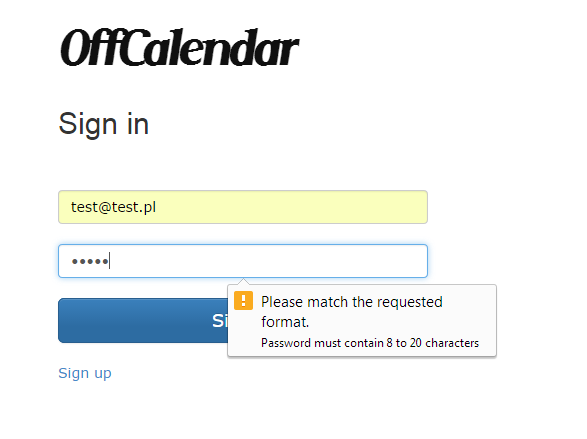
\includegraphics[width=0.5\textwidth]{signin.png}
\caption{Widok logowania użytkownika z przykładowym komunikatem ze standardu HTML5.}
\end{figure}

\begin{figure}[H]
\centering
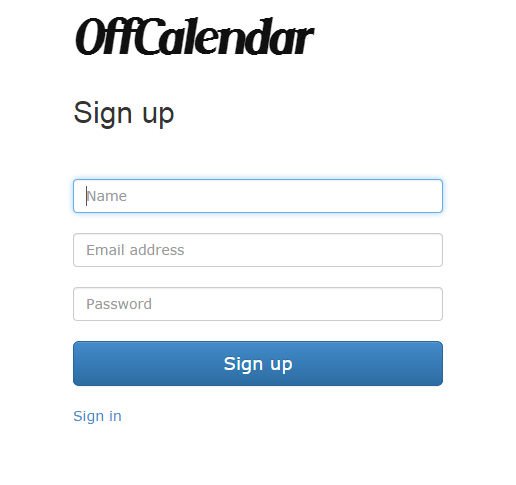
\includegraphics[width=0.5\textwidth]{register.png}
\caption{Widok rejestracji użytkownika.}
\end{figure}

Po pomyślnym utworzeniu konta i autoryzacji użytkownik zostaje przekierowany do głównego widoku aplikacji \textbf{dashboard}. Został on skonstruowany w taki sposób, aby załadować wszystkie potrzebne dane przy pierwszym wyświetleniu. Za pomocą atrybutu CSS \textbf{display: none} ukryto poszczególne sekcje. Przechodzenie pomiędzy nimi w menu polega na zmianie w/w atrybutu.

Główną część widoku zajmuje kalendarz wraz z przyciskami nawigacyjnymi. Utworzone wydarzenia możemy przeglądać na kilka określonych sposobów:

\begin{itemize}
\item w widoku rocznym z liczbą wydarzeń przypadających na dany miesiąc,
\item w widoku miesięcznym z graficzną reprezentacją wydarzeń z podziałem na dni miesiąca,
\item w widoku tygodniowym obrazującym harmonogram wraz z czasami trwania danych wydarzeń,
\item w widoku dziennym obrazującym wydarzenia wraz z godzinami rozpoczęcia oraz zakończenia.
\end{itemize}

W projekcie wykorzystano plugin \textbf{bootstrap-calendar}\footnote{\url{https://github.com/Serhioromano/bootstrap-calendar}}. Został on na potrzeby projektu rozszerzony o kompletny mechanizm dodawania, edycji oraz usuwania wydarzeń.

Oprócz przycisków nawigacyjnych, przenoszących pomiędzy widokami, w przestrzeni roboczej umieszczono przycisk \textbf{Add event} kierujący do widoku dziennego, gdzie istnieje możliwość dodawania nowych wydarzeń i edycji/usuwania istniejących. Rysunek 4.3 obrazuje formularz dodawania nowego wydarzenia wraz z wcześniej utworzonym wydarzeniem w widoku dziennym.

\begin{figure}[H]
\centering
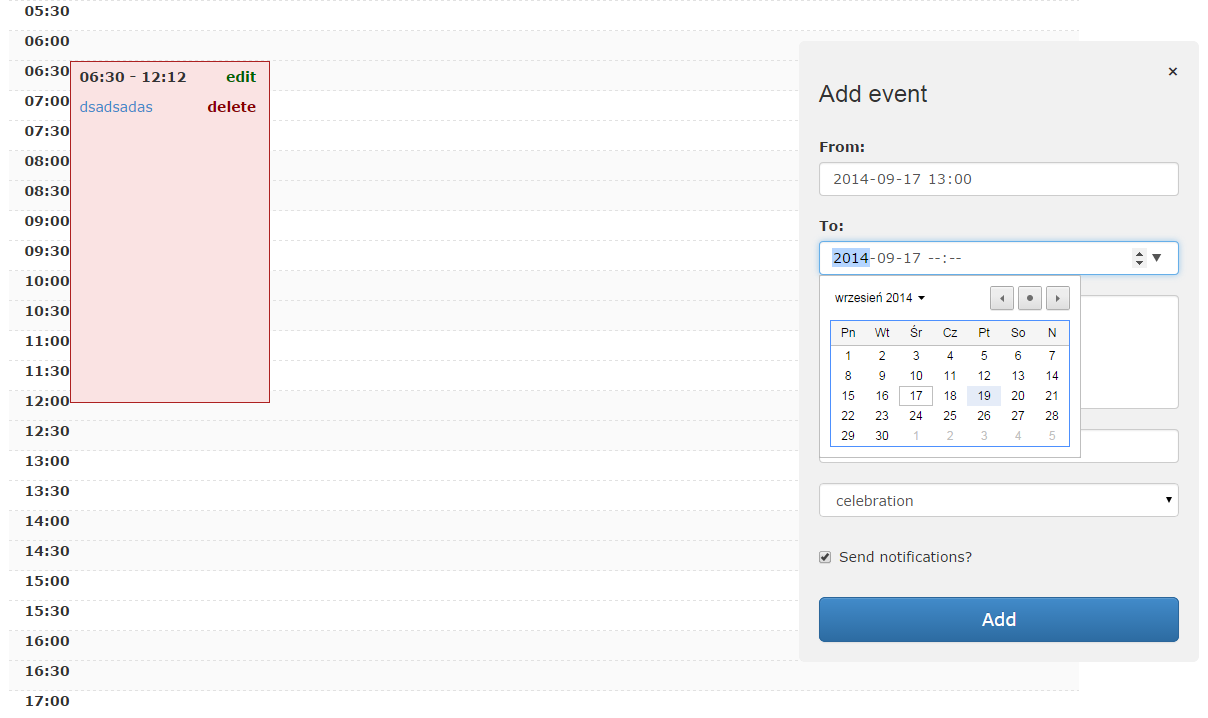
\includegraphics[width=0.9\textwidth]{add_event.png}
\caption{Formularz dodawania nowego wydarzenia w widoku dziennym.}
\end{figure}

Więcej nt. zarządzania wydarzeniami w sekcji 4.1.2.

Inicjacja kalendarza odbywa się w momencie załadowania widoku dashboard poprzez wywołanie metody \textbf{calendar}. Jako parametr przyjmuje ona opcje oraz kontekst. Opcje oznaczają parametry z jakimi wywołany zostanie kalendarz. Należą do nich m. in.

\begin{itemize}
\item szerokość kontenera,
\item widok początkowy (roczny, miesięczny, tygodniowy lub dzienny),
\item typ źródła danych (tablica, plik JSON, zewnętrzny plik),
\item ścieżka do katalogu zawierającego szablony widoków etc.
\end{itemize}

Kontekst definiowany jest przez element kodu HTML o określonym identyfikatorze (np. <div id=''kalendarz''></div>) w którym umieszczony zostanie kalendarz.

Widoki kalendarza ładowane są asynchroniczne. Zostały skonstruowane w HTML z zastosowaniem silnika szablonów JavaScript o nazwie \textbf{Underscore.js}\cite{underscore}. Separuje on warstwę danych od warstwy prezentacji i dostarcza wielu funkcji pozwalających operować na przekazanych do widoku zmiennych. Poniższy (Listing 4.4) fragment uproszczonego kodu z widoku dziennego obrazuje prostą pętlę wyświetlającą wydarzenia.

\begin{lstlisting}[caption=Fragment kodu prezentujący składnię Underscore.js., label=amb, captionpos=b]

<% _.each(after_time, function(event){ %>
<div class="day-highlight dh-<%= event.class %>">
       		<span class="cal-hours"><%= event.start_hour %></span>
              	<%= event.description %></a>
       </div>
<% }); %>

\end{lstlisting}

Prócz głównego widoku kalendarza użytkownik ma możliwość przejścia do następujących sekcji:

\begin{itemize}
\item \textbf{Upcoming events:} lista wydarzeń nadchodzących,
\item \textbf{Ongoing events:} lista wydarzeń trwających,
\item \textbf{Past events:} lista wydarzeń zakończonych,
\item \textbf{Your profile:} dane użytkownika wraz z liczbą stworzonych wydarzeń oraz liczbą wydarzeń z aktywowanymi powiadomieniami.
\end{itemize}

Dodatkowo zaimplementowano uproszczony mechanizm wyszukiwania wydarzeń po treści. Kod funkcji \textbf{initSearch()} przedstawiono na listingu 4.5.

\begin{lstlisting}[caption=Wyszukiwanie wydarzeń w oparciu o treść., label=amb, captionpos=b]

OffCalendar.initSearch = function () {

    $(document).ready(function () {
    
        var $form = $('form[name=search_event]');

        $form.submit(function (event) {

            event.preventDefault();

            var userId = OffCalendar.user.id;
            var formData = $form.serializeArray();
            var searchTerm = formData[0]['value'];

            if (searchTerm !== '') {

                IndexedDB.searchEvent(userId, searchTerm, function (events) {

                    var $containers = $('.offcalendar-container');
                    var $searchContainer = $('#search-cont');

                    OffCalendar.appendEventsHTML($searchContainer, events);

                    $containers.hide();
                    $searchContainer.show();
                });
            }
        });
    });
};

\end{lstlisting}

Po zakończeniu pracy z aplikacją OffCalendar następuje wylogowanie (\textbf{Logout}), co w praktyce wiąże się z usunięciem zapisanych w obiekcie localStorage danych logowania.

\subsection{Zarządzanie wydarzeniami}
\label{sec:zarzWyd}

Ogół operacji związanych z manipulacją wydarzeniami (dodawanie, edycja oraz usuwanie) spoczywa na mechanizmie \textbf{IndexedDB}. Inicjacja obiektu bazy lokalnej następuje w momencie każdorazowego ładowania widoku dashboard. Listing 4.6 obrazuje otwarcie połączenia z bazą danych.

\begin{lstlisting}[caption=Otwarcie połączenia z lokalną bazą danych., label=amb, captionpos=b]

IndexedDB.open = function (callback) {

    var request = indexedDB.open(DB_NAME, DB_VERSION);

    request.onupgradeneeded = function (e) {

        var db = e.target.result;

        e.target.transaction.onerror = IndexedDB.onerror;

        if (db.objectStoreNames.contains(DB_STORE_NAME)) {
            db.deleteObjectStore(DB_STORE_NAME);
        }

        var store = db.createObjectStore(DB_STORE_NAME, {keyPath: "remote_id", autoIncrement: true});

        store.createIndex('id', 'id', {unique: true});
        store.createIndex('user_id', 'user_id', {unique: false});
        store.createIndex('voided', 'voided', {unique: false});
        store.createIndex('remote_timestamp', 'remote_timestamp', {unique: false});
        store.createIndex('search', ['user_id', 'description'], {unique: false});

    };

    request.onsuccess = function (e) {
        IndexedDB.db = e.target.result;
        callback(true);
    };

    request.onerror = function (event) {
        callback(false);
    };
};

\end{lstlisting}

Baza lokalna zostaje otwarta z dwoma parametrami: nazwą bazy oraz jej wersją. Następnie tworzone są indeksy niezbędne do przeszukiwania po nazwach pól np. indeks o nazwie \textbf{search} wyszukuje pola \textbf{user\_id} oraz \textbf{description} i akceptuje duplikaty. Zarówno w przypadku pomyślnego jak i błędnego wykonania żądania wykonywana jest funkcja określona w parametrze callback. 

W aplikacji OffCalendar po otwarciu połączenia do bazy danych wykonywane jest pobranie wydarzeń dla danego użytkownika (Listing 4.7) a następnie zainicjowanie synchronizacji

\begin{lstlisting}[caption=Pobranie wydarzeń użytkownika., label=amb, captionpos=b]

IndexedDB.getUserEvents = function (userId, callback) {

    var resultSet = [];

    var transaction = IndexedDB.db.transaction([DB_STORE_NAME], DB_TRANS_MODE_READ_ONLY);

    var store = transaction.objectStore(DB_STORE_NAME);

    var keyRange = IDBKeyRange.only(userId);

    var cursorRequest = store.index('user_id').openCursor(keyRange);

    cursorRequest.onsuccess = function (e) {

        var result = e.target.result;

        if (!!result === false)
            return;

        resultSet.push(result.value);

        result.continue();
    };

    transaction.oncomplete = function (event) {
        callback(resultSet);
    };

    cursorRequest.onerror = function (event) {
        callback(null);
    };
};

\end{lstlisting}

Flaga DB\_STORE\_NAME oznacza nazwę tabeli, natomiast DB\_TRANS\_MODE\_ONLY tryb dostępu (w tym przypadku wyłącznie odczyt). Następnie wykorzystywany jest indeks tworzony wraz z nową wersją bazy danych. Obiekt \textbf{cursorRequest} pozwala przeszukiwać tabelę i zapisywać rekordy (spełniające warunki określone w indeksie) do tablicy wynikowej \textbf{resultSet} wykorzystanej następnie w funkcji callback.

Pobrane wydarzenia zostają zapisane w opcjach kalendarza, po czym następuje jego renderowanie. Strukturę obiektu reprezentującego przykładowe wydarzenie przedstawia listing 4.8:

\begin{lstlisting}[caption=Struktura obiektu reprezentującego wydarzenie., label=amb, captionpos=b]

class: "event-important"
start_timestamp: 1411349400000
end_timestamp: 1411380720000
last_update_timestamp: 0
remote_id: 1
remote_timestamp: 1411398325288
send_notification: 0
description: "test"
url: ""
user_id: 4
voided: 0

\end{lstlisting}

Poszczególne pola oznaczają kolejno: klasę wydarzenia (kolor), stempel czasowy rozpoczęcia wydarzenia, stempel czasowy zakończenia wydarzenia, stempel czasowy ostatniej synchronizacji (0 oznacza nowo dodane wydarzenie), identyfikator rekordu, stempel czasowy ostatniej aktualizacji wydarzenia przez użytkownika, flagę informującą o wysyłaniu powiadomień \mbox{e-mail}, opis wydarzenia, zewnętrzny adres url, id użytkownika oraz flagę informującą o usunięciu danego wydarzenia (ustawiona na wartość 1 oznacza, że użytkownik usunął wydarzenie).

Dodawanie, edycja oraz usuwanie wydarzeń odbywa się widoku dziennym. Przedstawia on godziny dnia w odstępie 30 minutowym. Kliknięcie na każdą z nich otwiera okno dodawania nowego wydarzenia z odpowiednio uzupełnioną datą rozpoczęcia. W przypadku edycji wydarzenia to samo okno zostaje uzupełnione również o wszystkie pozostałe dane wydarzenia. Poniższy kod (Listing 4.9) obrazuje operację edycji.

\begin{lstlisting}[caption=Edycja wydarzenia cz. 1., label=amb, captionpos=b]

IndexedDB.updateEvent = function (eventRemoteId, eventPropertiesToUpdate, callback) {

    var trans = IndexedDB.db.transaction([DB_STORE_NAME], DB_TRANS_MODE_READ_WRITE);

    var store = trans.objectStore(DB_STORE_NAME);

    var cursorRequest = store.openCursor(IDBKeyRange.only(eventRemoteId));

    cursorRequest.onsuccess = function (e) {

        var cursor = cursorRequest.result || e.result;

        var Event = cursor.value;

        for (var property in eventPropertiesToUpdate) {
            Event[property] = eventPropertiesToUpdate[property];
        }

        var request = cursor.update(Event);

        request.onerror = function (e) {
            callback(null);
        };

        request.onsuccess = function (e) {
            callback(Event);
        };
    };
};

\end{lstlisting}

W przypadku poprawnego dodania wydarzenia wykonywana jest funkcja callback. W aplikacji \mbox{OffCalendar} użytkownik zostanie poinformowany o efekcie żądania i przekierowany na stronę główną. Następny listing (4.10) obrazuje operację pobrania danych z formularza edycji wydarzenia i przekazania ich do powyższej funkcji oraz przekierowanie realizowane z użyciem odpowiedniej funkcji zwrotnej.

\begin{lstlisting}[caption=Edycja wydarzenia cz. 2., label=amb, captionpos=b]

OffCalendar.initEventUpdate = function () {

    var $form = $('form[name=offcalendar_update_event]');

    $form.submit(function (event) {

        event.preventDefault();

        var formData = $form.serializeArray();

        var userId = OffCalendar.user.id;

        var startTimestamp = OffCalendarHelper.getTimestampFromDate(formData[0]['value']);
        var endTimestamp = OffCalendarHelper.getTimestampFromDate(formData[1]['value']);

        var description = formData[2]['value'];

        var url = formData[3]['value'];
        var eventClass = OffCalendarHelper.mapEventTypeToClassName(formData[4]['value']);

        var sendNotification = $('input#send_notification').is(':checked');

        var toUpdate = {
            user_id: userId,
            start_timestamp: startTimestamp,
            end_timestamp: endTimestamp,
            description: description,
            url: url,
            class: eventClass,
            send_notification: sendNotification ? 1 : 0,
            voided: 0,
            remote_timestamp: OffCalendarHelper.currentTimestamp()
        };

        var eventRemoteId = formData[5]['value'];
        eventRemoteId = parseInt(eventRemoteId, 10);

        IndexedDB.updateEvent(eventRemoteId, toUpdate, function (Event) {
            if (Event !== null) {
                OffCalendar.showFlashMessage('success', 'Event succesfully updated!', function () {
                    window.location = OffCalendar.dashboardUrl;
                });
            }
        });
    });

};

\end{lstlisting}

Dodawanie wydarzenia wykonywane jest analogicznie. Z kolei operacja usuwania polega na zmianie atrybutu \textbf{voided} na wartość 1. Jest to konieczne z uwagi na synchronizację wydarzeń pomiędzy różnymi urządzeniami: całkowite usunięcie konkretnego obiektu z bazy lokalnej mogłoby prowadzić do konfliktów.

Pozostałe operacje związane z manipulacją wydarzeniami sprowadzają się do pobrania tablicy obiektów \textbf{Event}, analizy pod względem daty rozpoczęcia i zakończenia oraz klasyfikacji poprzez umieszczenie w jednej z sekcji dostępnych w menu (Past Events, Ongoing Events, Upcoming Events).

Zarówno dodawanie, usuwanie jak i edycja wydarzenia kończy się przekierowaniem do głównej strony aplikacji i wywołaniem synchronizacji z częścią serwerową poprzedzoną weryfikacją obecności połączenia internetowego.

\subsection{Detekcja połączenia internetowego}
\label{sec:detPolInt}

W związku z faktem, że aplikacja OffCalendar oferuje również wsparcie dla trybu online, automatyczna detekcja stanu połączenia internetowego jest kluczowa. Posiadanie dostępu do sieci Internet umożliwia autoryzację oraz, co najważniejsze, synchronizację danych lokalnych z główną bazą będącą częścią części serwerowej projektu.

W aplikacji zastosowano bibliotekę Offline.js \footnote{\url{http://github.hubspot.com/offline/docs/welcome/}}. Oferuje ona automatyczną detekcję połączenia wraz z powiadomieniami o jego stanie oraz możliwość wykonania próby jego ponowienia. Wraz z logiką biblioteki twórcy zaproponowali szablony komunikatów podlegające pełnej personalizacji.

Działanie biblioteki opiera się na cyklicznym wykonywaniu żądania AJAX pobrania niewielkiego zasobu graficznego (1x1 pikseli) w formacie png o rozmiarze 110 bajtów. Wybór ten umożliwia odwołanie do zasobu znajdującego się pod innym adresem, ponieważ koncepcja \textbf{Same-origin policy}\footnote{Same-origin policy, inaczej zasada tożsamego pochodzenia, zezwala na dostęp do zasobów stron, których adres wyróżnia się takim samym protokołem, nazwą domeny serwera i numerem portu\cite{sameOrigin}} nie odnosi się do obiektów graficznych.

Inicjacja biblioteki wykonywana jest w momencie załadowania widoku głównego. Polega ona na podaniu kilku opcji przedstawionych na listingu 4.11.

\begin{lstlisting}[caption=Inicjalizacja biblioteki Offline.js badającej stan połączenia internetowego., label=amb, captionpos=b]

Offline.options = {
	checks: {
   	   image: {
            url: '[adres_url]/blank.png?_=' + (Math.floor(Math.random() * 1000000000))
       },
       active: 'image'
    },
    reconnect: false,
    checkOnLoad: true
};

\end{lstlisting}

\begin{itemize}
\item \textbf{url:} oznacza adres zasobu graficznego; dodany kod oblicza pseudo-losowy numer i dokleja go do adresu url żądania, celem uniknięcia cache-owania wskazanego pliku png,
\item \textbf{active:} oznacza typ zasobu - biblioteka oferuje bowiem również sprawdzanie stanu połączenia w oparciu o skrypt,
\item \textbf{reconnect:} flaga informująca o konieczności ponawiania połączenia - w projekcie zbędna z uwagi na fakt, że dysponowanie aktywnym połączeniem sieciowym nie jest konieczne do prawidłowego funkcjonowania aplikacji,
\item \textbf{checkOnLoad:} flaga informująca o konieczności wykonania testu połączenia w momencie załadowania widoku głównego.
\end{itemize}

Żądanie opiera się na właściwościach obiektu \textbf{XMLHttpRequest} zapewniających asynchroniczne wykonanie, czyli bez przeładowania strony. Poniżej (Listing 4.12) kod głównej metody checkXHR(xhr, onUp, onDown) sprawdzającej stan połączenia internetowego w oparciu o opcje obiektu XMLHttpRequest (xhr) ustawione w momencie inicjalizacji biblioteki i wywołującego funkcje callback.

\begin{lstlisting}[caption=Metoda checkXHR() wykonująca żądanie AJAX załadowania zasobu graficznego., label=amb, captionpos=b]
checkXHR = function(xhr, onUp, onDown) {
        var checkStatus, _onerror, _onload, _onreadystatechange, _ontimeout;
        checkStatus = function() {
            if (xhr.status && xhr.status < 12000) {
                return onUp();
            } else {
                return onDown();
            }
        };
        if (xhr.onprogress === null) {
            _onerror = xhr.onerror;
            xhr.onerror = function() {
                onDown();
                return typeof _onerror === "function" ? _onerror.apply(null, arguments) : void 0;
            };
            _ontimeout = xhr.ontimeout;
            xhr.ontimeout = function() {
                onDown();
                return typeof _ontimeout === "function" ? _ontimeout.apply(null, arguments) : void 0;
            };
            _onload = xhr.onload;
            return xhr.onload = function() {
                checkStatus();
                return typeof _onload === "function" ? _onload.apply(null, arguments) : void 0;
            };
        } else {
            _onreadystatechange = xhr.onreadystatechange;
            return xhr.onreadystatechange = function() {
                if (xhr.readyState === 4) {
                    checkStatus();
                } else if (xhr.readyState === 0) {
                    onDown();
                }
                return typeof _onreadystatechange === "function" ? _onreadystatechange.apply(null, arguments) : void 0;
            };
        }};
\end{lstlisting}

Tylko w sytuacji, w której połączenie internetowe jest aktywne wykonywana jest synchronizacja wydarzeń. Poniżej wygląd komunikatów informujących o pracy w trybie online/offline (odpowiednio rysunki 4.4 oraz 4.5).

\begin{figure}[H]
\centering
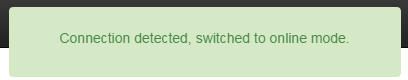
\includegraphics[width=0.9\textwidth]{isOnline.png}
\caption{Komunikat o przejściu w tryb online.}
\end{figure}

\begin{figure}[H]
\centering

\includegraphics[width=0.9\textwidth]{isOffline.png}
\caption{Komunikat o przejściu w tryb offline.}
\end{figure}

\subsection{Synchronizacja danych}
\label{autSynDanych}

Proces synchronizacji danych jest uruchamiany co 3 minuty, a także po dodaniu, edycji lub usunięciu wydarzenia. Proces rozpoczyna się w momencie wywołania metody synchronize (Listing 4.13). Do funkcji przekazane są dane użytkownika, adres URL interfejsu programowania odpowiedzialnego za proces po stronie serwerowej aplikacji oraz funkcja, która zostanie wywołana po zakończeniu synchronizacji.

\begin{lstlisting}[caption=Funkcja synchronize rozpoczynająca proces synchronizacji., label=amb, captionpos=b]
IndexedDB.synchronize = function(userId, userEmail, userPassword, eventsSyncApiUrl, callback) {

	if (IndexedDB.sync.inProgress === true) {
    	return;
	}

	IndexedDB.sync.inProgress = true;
	IndexedDB.sync.userId = userId;
	IndexedDB.sync.remoteTimestamp = OffCalendarHelper.currentTimestamp();
	IndexedDB.sync.itemsSynced = 0;
	IndexedDB.sync.email = userEmail;
	IndexedDB.sync.password = userPassword;
	IndexedDB.sync.url = eventsSyncApiUrl;
	IndexedDB.sync.callback = callback;

	var lastRemoteSyncTimestamp = IndexedDB.sync.getLastRemoteSyncTimestamp(userId);

	IndexedDB.getUserEventsForSync(userId, lastRemoteSyncTimestamp, IndexedDB.sync.eventsFetched);


};
\end{lstlisting}

W przypadku gdy proces synchronizacji jest w trakcie wykonania (atrybut  IndexedDB.sync.inProgress posiada wartość true) kolejne wywołania metody będą odwoływane aż do chwili zakończenia procesu synchronizacji. Metoda ta pobiera stempel czasowy ostatniej synchronizacji oraz wydarzenia które zostały zmodyfikowane od czasu ostatniej synchronizacji.

Po pomyślnym pobraniu wydarzeń tworzone jest zapytanie AJAX wysyłające je do części serwerowej w celu ich synchronizacji (Listing 4.14).

\begin{lstlisting}[caption=Wysłanie żądania synchronizacji do części serwerowej., label=amb, captionpos=b]

IndexedDB.sync.eventsFetched = function(events) {

	if (events === null) {
    	IndexedDB.sync.failed('Error fetching events from db.');
	}

	var lastSyncTimestamp = IndexedDB.sync.getLastSyncTimestamp();

	var request = $.ajax({
    	url: IndexedDB.sync.url,
    	dataType: "json",
    	type: "POST",
    	data: {
        	email: IndexedDB.sync.email,
        	password: IndexedDB.sync.password,
        	last_sync_timestamp: lastSyncTimestamp,
        	events: JSON.stringify(events)
    	}
	});

	request.done(function(response, textStatus, jqXHR) {

    	IndexedDB.sync.processData(response);

	});

	request.fail(function(jqXHR, textStatus, errorThrown) {

    	var msg;

    	if (jqXHR.responseJSON && jqXHR.responseJSON.error) {
        	msg = jqXHR.responseJSON.error;
    	} else {
        	msg = jqXHR.status + ' - ' + errorThrown;
    	}

    	IndexedDB.sync.failed(msg);

	});

};
\end{lstlisting}

Część serwerowa zwraca zsynchronizowaną listę wydarzeń. Wydarzenia te zostają zaktualizowane w lokalnej bazie danych. Poniżej (Listing 4.15) przedstawiona jest funkcja dokonująca aktualizacji.

\begin{lstlisting}[caption=Aktualizacja wydarzeń przechowywanych w lokalnej bazie danych., label=amb, captionpos=b]

IndexedDB.sync.updateEvents = function() {

	if (IndexedDB.sync.eventsToUpdate.length > 0) {

    	var Event = IndexedDB.sync.eventsToUpdate.pop();

    	if (Event.id) {
        	IndexedDB.updateEventById(Event.id, Event, IndexedDB.sync.updateEvents);
    	} else {
        	IndexedDB.updateEvent(Event.remote_id, Event, IndexedDB.sync.updateEvents);
    	}

    	IndexedDB.sync.itemsSynced++;

	} else {

    	IndexedDB.sync.success();

	}

};

\end{lstlisting}

Po zakończeniu aktualizacji proces synchronizacji dobiega końca (Listing 4.16). Przed zakończeniem konieczne jest zaktualizowanie stempli czasowych - zarówno wygenerowanego po stronie klienta jak i serwera.

\begin{lstlisting}[caption=Kod finalizujący proces synchronizacji., label=amb, captionpos=b]

IndexedDB.sync.success = function() {

	IndexedDB.sync.inProgress = false;

	IndexedDB.sync.setLastRemoteSyncTimestamp(IndexedDB.sync.remoteTimestamp);
    
	IndexedDB.sync.setLastSyncTimestamp(IndexedDB.sync.timestamp);

	IndexedDB.sync.callback(IndexedDB.sync.itemsSynced);

};

\end{lstlisting}

Po wykonaniu aktualizacji stempli oraz zaktualizowaniu flagi wskazującej na to, że proces synchronizacji jest w toku wywoływana jest, przekazana na początku procesu, funkcja. Jej argumentem jest ilość wydarzeń które zostały zsynchronizowane.

\section{Aplikacja serwerowa}
\label{sec:apSerw}

Aby aplikacja OffCalendar działała prawidłowo, konieczna była implementacja mechanizmów dostępu do bazy danych i zarządzania danymi oraz implementacja bezstanowych interfejsów odpowiadających za komunikację z częścią kliencką aplikacji.

Największym problemem, który należało rozwiązać, były różnice w strukturze obiektów przechowywanych po stronie klienckiej oraz serwerowej. Mechanizmy odpowiedzialne za zarządzanie wydarzeniami musiały zostać zaimplementowane w taki sposób, aby umożliwiały łatwą konwersję oraz porównywanie różnych typów wydarzeń.

\subsection{Implementacja warstwy danych}
\label{komBazaDanych}

Pierwszym z elementów, który musiał zostać wykonany w części serwerowej aplikacji była warstwa danych. Składają się na nią: 

\begin{enumerate}
\item klasy wykonujące operacje CRUD oparte na klasie ActiveRecord\cite{ciActiveRecord} frameworku CodeIgniter:
\begin{itemize}
\item \textbf{Events\_model}
\item \textbf{Users\_model}
\end{itemize}
\item klasy służące do mapowania rekordów przechowywanych w bazach danych (klienckiej oraz serwerowej) na poszczególne obiekty:
\begin{itemize}
\item \textbf{Event}
\item \textbf{User}
\end{itemize}
\end{enumerate}

Wydarzenia (Event) są tworzone po stronie aplikacji klienckiej i każdemu z nich jest przypisywana unikalna wartość lokalnego klucza głównego. Dodatkowo każde wydarzenie przechowywane w bazie danych posiada również klucz główny generowany przez bazę danych. Z tego względu, przy inicjalizacji oraz zapisie do bazy danych obiektów wydarzeń, powyższe różnice musiały zostać odpowiednio obsłużone.

Dobrym przykładem jest kod konstruktora klasy Event (Listing 4.17), który sprawdza obecność obydwu kluczy głównych i na ich podstawie odpowiednio inicjuje obiekt.

\definecolor{dkgreen}{rgb}{0,.6,0}

\lstset{
  language        = php,
  basicstyle      = \small\ttfamily,
  keywordstyle    = \color{blue},
  stringstyle     = \color{orange},
  identifierstyle = \color{dkgreen},
  commentstyle    = \color{gray},
  emph            =[1]{php},
  emphstyle       =[1]\color{black},
  emph            =[2]{__construct,int,string,public,private,function,try,throw,catch,\$this,return,if,and,or,else,foreach},
  emphstyle       =[2]\color{blue},
  showstringspaces=false
}

\begin{lstlisting}[caption=Fragment konstruktora klasy Event., label=amb, captionpos=b]

public function __construct($properties = array()) {
    if ($properties) {
        if (isset($properties['id']) && $properties['id']) {
            $this->id = (int) $properties['id'];
        }

        if (isset($properties['remote_id']) && $properties['remote_id']) {
            $this->remoteId = (int) $properties['remote_id'];
        }

        $this->userId = (int) $properties['user_id'];
        $this->startTimestamp = (int) $properties['start_timestamp'];
        $this->endTimestamp = (int) $properties['end_timestamp'];
        $this->description = (string) $properties['description'];
        $this->sendNotification = (int) $properties['send_notification'];
        $this->voided = (int) $properties['voided'];
        $this->remoteTimestamp = (int) $properties['remote_timestamp'];
        $this->lastUpdateTimestamp = (int) $properties['last_update_timestamp'];
    }
}

\end{lstlisting}

W zależności czy dane wydarzenie ma zostać zapisane w bazie danych czy też zwrócone do aplikacji klienckiej, musi ono zawierać odpowiedni zestaw atrybutów. Do tego celu stworzone zostały poniższe metody klasy Event (Listing 4.18).

\begin{lstlisting}[caption=Serializacja obiektu Event., label=amb, captionpos=b]

public function toDbArray() {
    return array(
        'user_id' => $this->userId,
        'start_timestamp' => $this->startTimestamp,
        'end_timestamp' => $this->endTimestamp,
        'description' => $this->description,
        'send_notification' => $this->sendNotification,
        'voided' => $this->voided,
        'remote_timestamp' => $this->remoteTimestamp,
        'last_update_timestamp' => $this->lastUpdateTimestamp,
    );
}

public function toApiArray() {
    $arr = $this->toDbArray();

    $additional = array(
    	'id' => $this->id,
    );

    if ($this->remoteId) {
    	$additional['remote_id'] = $this->remoteId;
    }

    return array_merge($additional, $arr);
}

\end{lstlisting}

Dla wydarzeń posiadających klucz główny wygenerowany w bazie danych, aktualizacja dokonywana jest na jego podstawie. W przeciwnym wypadku dla danego wydarzenia utworzony zostaje nowy rekord w bazie danych (kod z listingu 4.19).

\begin{lstlisting}[caption=Aktualizacja obiektu Event w bazie danych., label=amb, captionpos=b]

function persist() {
   	if ($this->id) {
       		$this->_ci->events_model->updateEvent($this->id, $this->toDbArray());
   	} else {
       		$this->id = $this->_ci->events_model->addEvent($this->toDbArray());
   	}

   	return $this;
}

\end{lstlisting}

Klasa Events\_model bezpośrednio odpowiada za manipulację rekordami znajdującymi się w bazie danych. Bogaty zbiór metod klasy ActiveRecord pozwala na łatwe wykonanie operacji tworzenia, pobierania oraz aktualizacji rekordów (Listing 4.20).

\begin{lstlisting}[caption=Przykładowe metody klasy Events\_model odpowiedzialne za komunikację z bazą danych., label=amb, captionpos=b]

function getEventById($eventId) {
	
   $query = $this->db->get_where('events', array('id' => $eventId));

   return $query->row_array();
}

function updateEvent($eventId, $toUpdate) {

   $this->db->update('events', $toUpdate, array('id' => $eventId));

   return $this->db->affected_rows();
}

function addEvent($event) {
   	
   $this->db->insert('events', $event);

   return $this->db->insert_id();
}

\end{lstlisting}

Klasy User oraz Users\_model zostały stworzone analogicznie do klas Events oraz Events\_model. Różnicą jest tutaj brak klucza głównego generowanego po stronie klienta. Wynika to z faktu, iż konta użytkowników mogą być tworzone wyłącznie w trybie online. Pozwala to na uniknięcie narzutu spowodowanego koniecznością przechowywania podwójnych kluczy głównych.

\subsection{Bezstanowe interfejsy}
\label{bezstInter}

W celu komunikacji z częścią kliencką stworzone zostały interfejsy programowania aplikacji umożliwiające manipulację danymi użytkowników oraz synchronizację wydarzeń. Ze względu na nacisk położony na tryb offline interfejsy zostały stworzone zgodnie z zasadami architektury REST. W celu minimalizacji danych przesyłanych do klienta, odpowiedzi zawierają dane w formacie JSON.

Większość metod używanych przez interfejsy wymaga wcześniejszej autentykacji użytkownika. Wyjątkiem jest tutaj metoda register interfejsu Users\_api pozwalająca na rejestrację nowych użytkowników.

\begin{lstlisting}[caption=Rejestracja użytkowników przy użyciu metody register interfejsu Users\_api., label=amb, captionpos=b]

function register() {
  try {
      if (!$this->input->post()) {
      	throw new Exception('Please fill required fields');
      }

      $fields = $this->users->getFieldsValidationRules(array('name', 'email', 'password'));

      $this->form_validation->set_rules($fields);

      if (!$this->form_validation->run()) {
      	throw new Exception(strip_tags(validation_errors()));
      }

      $vals = array();

      foreach (array_keys($fields) as $f) {
      	$vals[] = $this->form_validation->set_value($f);
      }

      list($name, $email, $password) = $vals;

      $user = $this->users->register($name, $email, $password);

      return $this->jsonResponse($user->toApiResponse());
  } catch (Exception $e) {
      return $this->jsonError($e->getMessage());
  }
}

\end{lstlisting}

Metoda register (Listing 4.21) w pierwszej kolejności sprawdza poprawność danych przesłanych przez aplikację kliencką. W przypadku błędu do aplikacji klienckiej zwracana jest odpowiednia wiadomość oraz kod błędu. Po pomyślnym utworzeniu nowego konta, odpowiedź zawiera  dane użytkownika, w których znajduje się m. in. jego unikalny identyfikator, na podstawie którego można zidentyfikować przechowywane w lokalnej bazie danych rekordy do niego należące.

Wspólną dla wszystkich interfejsów programowania jest funkcja odpowiadająca za autentykację użytkownika. Ze względu na bezstanowość, przy każdym żądaniu synchronizacji danych czy aktualizacji danych użytkownika, konieczne jest potwierdzenie jego tożsamości.

\begin{lstlisting}[caption=Rejestracja użytkowników przy użyciu metody register interfejsu Users\_api., label=amb, captionpos=b]

private function authenticateUser() {
  try {
	$email = (string) $this->input->post('email');

	$password = (string) $this->input->post('password');

	$user = $this->users->login($email, $password);

    return $user;
  } catch (Exception $e) {
	throw new Exception('Authentication failed.');
  }
}

\end{lstlisting}

Powyższa metoda (Listing 4.22) w przypadku pomyślnej autentykacji zwraca obiekt User, natomiast w przypadku niezgodności przesłanych danych rzucany jest odpowiedni wyjątek informujący, że proces autentykacji się nie powiódł.

\subsection{Synchronizacja danych}
\label{serwSynDanych}

Najbardziej złożonym procesem wykonywanym w aplikacji OffCalendar jest synchronizacja danych. Część serwerowa tego procesu rozpoczyna się w momencie przesłania przez część kliencką żądania synchronizacji. Żądanie musi zawierać dane wymagane do autentykacji użytkownika, stempel czasowy określający czas ostatniej synchronizacji oraz listę wydarzeń, które uległy modyfikacji od czasu ostatniej synchronizacji.

\begin{lstlisting}[caption=Metoda synchronize interfejsu programowania Events\_api., label=amb, captionpos=b]
function synchronize() {
   	try {
	   $user = $this->authenticateUser();

       $userId = $user->getId();

       $lastSyncTimestamp = (int)$this->input->post('last_sync_timestamp');
       $currTimestamp = time();

       $dbEvents = $this->events->getDbEventsForSynchronization($userId, $lastSyncTimestamp);       	 
       $postEvents = $this->input->post('events');

       $remoteEvents = $this->events->getEventsFromPostData($postEvents, $user);
      	 
       $eventsToUpdate = $this->events->synchronize($remoteEvents, $dbEvents, $currTimestamp);

       $toUpdate = array();
       	 
       foreach($eventsToUpdate as $e){
          $toUpdate[] = $e->toApiArray();
       }

       $response = array(
          'sync_timestamp' => $currTimestamp,
          'events_to_update' => $toUpdate,
       );

       return $this->jsonResponse($response);
    } catch (Exception $e) {

      return $this->jsonError($e->getMessage());
  }
}

\end{lstlisting}

Powyższa metoda (Listing 4.23) sprawdza poprawność przesłanych przez część kliencką danych oraz przekazuje komponentowi Events dane potrzebne do poprawnej modyfikacji wydarzeń. Komponent Events zwraca listę zaktualizowanych wydarzeń, które zostaną przesłane do części klienckiej celem aktualizacji wydarzeń w lokalnej bazie danych. Do odpowiedzi zostaje dołączony również stempel czasowy synchronizacji.

\begin{lstlisting}[caption=Modyfikacja wydarzeń w metodzie synchronize komponentu Events., label=amb, captionpos=b]

public function synchronize($remoteEvents, $dbEvents, $currTimestamp) {
   	$toUpdate = array();

   	foreach ($remoteEvents as $remoteEvent) {

      if (!$remoteEvent->hasId()) {

	      $remoteEvent->setLastUpdateTimestamp($currTimestamp);

          $remoteEvent->persist();

          $toUpdate[] = $remoteEvent;

          continue;
      }

      $eventId = $remoteEvent->getId();

      if (isset($dbEvents[$eventId])) {

          $dbEvent = $dbEvents[$eventId];

          if ($dbEvent->getRemoteTimestamp() > $remoteEvent->getRemoteTimestamp()) {
          	$dbEvent->setRemoteId($remoteEvent->getRemoteId());
            $toUpdate[] = $dbEvent;
          } else {
            $remoteEvent->setLastUpdateTimestamp($currTimestamp);
            $remoteEvent->persist();
            $toUpdate[] = $remoteEvent;
          }

          unset($dbEvents[$eventId]);
      }
    }

    foreach ($dbEvents as $dbEvent) {

       	$toUpdate[] = $dbEvent;
    }

   	return $toUpdate;
}

\end{lstlisting}

Metoda synchronize komponentu events, przedstawiona na listingu 4.24, dzieli wydarzenia na wyszczególnione na etapie projektu (3.3.3) kategorie. Wydarzenia przesłane przez część kliencką zawierają wartość klucza głównego wygenerowanego przez lokalną bazę danych co umożliwia wydajną aktualizację rekordów. W przypadku wydarzeń, które zostały zmodyfikowane na innym urządzeniu obecny jest jedynie klucz główny wygenerowany na serwerze. Na jego podstawie aplikacja kliencka musi zadecydować o stworzeniu nowego rekordu lub aktualizacji już istniejącego.
